% 图 2.15 顺磁盐熵 S(T) 曲线族（J=1/2 + T^3 晶格项），等温磁化 a->b 与绝热退磁 b->c
\documentclass[tikz,border=5pt]{standalone}
\usetikzlibrary{arrows.meta}
\usepackage{amsmath}
\usepackage{bm}
\usepackage{fontspec}
\setmainfont{Times New Roman}
\usepackage{pgfplots}
\pgfplotsset{compat=1.18}
\begin{document}
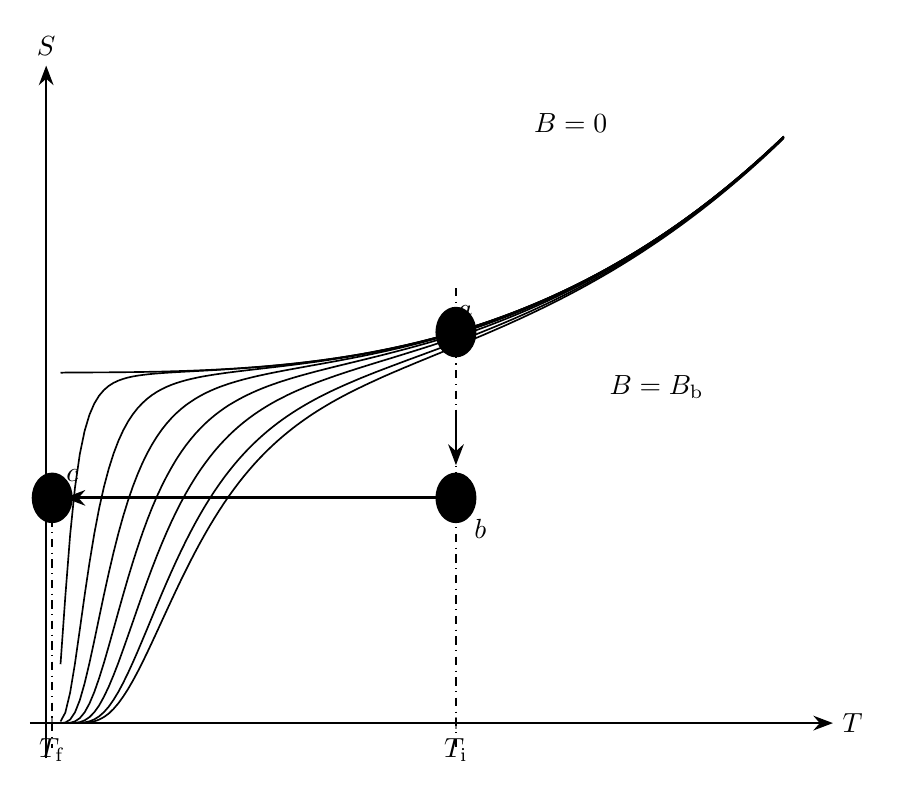
\begin{tikzpicture}[line width=0.8pt,>=Stealth]
% 曲线族
\begin{axis}[at={(0cm,0cm)},anchor=south west,
  width=10.2cm,height=8.8cm,scale only axis,
  axis lines=middle,
  axis line style={-Stealth,line width=0.9pt},
  xmin=-0.04,xmax=1.92,ymin=-0.07,ymax=1.30,
  xtick={0.0147,1.0},xticklabels={$T_{\mathrm{f}}$,$T_{\mathrm{i}}$},
  ytick=\empty,
  tick style={line width=0.7pt},
  xlabel={$T$},
  x label style={at={(axis cs:1.92,0)},anchor=west},
  ylabel={$S$},
  y label style={at={(axis cs:0,1.30)},anchor=south},
  clip=true]
  % S = ln(2 cosh(B/T)) - (B/T) tanh(B/T) + 0.08 T^3
  \foreach \B in {0.012,0.15,0.3,0.45,0.6,0.75,0.9,1.0}{
    \addplot[line width=0.6pt,domain=0.035:1.8,samples=151]
      {ln(exp(\B/x)+exp(-\B/x)) - (\B/x)*(exp(\B/x)-1)/(exp(\B/x)+1) + 0.08*x^3};
  }
\end{axis}
% 磁制冷路径与标注（叠加坐标系）
\begin{axis}[at={(0cm,0cm)},anchor=south west,
  width=10.2cm,height=8.8cm,scale only axis,
  axis lines=none,
  xmin=-0.04,xmax=1.92,ymin=-0.07,ymax=1.30,
  clip=false]
  \draw[dash dot,line width=0.55pt] (axis cs:1,0.86) -- (axis cs:1,-0.05);
  \draw[dash dot,line width=0.55pt] (axis cs:0.0147,0.4453) -- (axis cs:0.0147,-0.05);
  \draw[->,line width=1.0pt] (axis cs:1,0.62) -- (axis cs:1,0.51);
  \draw[->,line width=1.0pt] (axis cs:1,0.4453) -- (axis cs:0.0147+0.03,0.4453);
  \fill (axis cs:1,0.7731) circle (0.05);
  \fill (axis cs:1,0.4453) circle (0.05);
  \fill (axis cs:0.0147,0.4453) circle (0.05);
  \node[anchor=south west,inner sep=2pt] at (axis cs:0.99,0.7901) {$a$};
  \node[anchor=north west,inner sep=2pt] at (axis cs:1.03,0.4453-0.03) {$b$};
  \node[anchor=south west,inner sep=2pt] at (axis cs:0.0147+0.02,0.4453+0.02) {$c$};
  \node[anchor=south,inner sep=2pt] at (axis cs:1.28,1.155) {$B=0$};
  \node[anchor=north west,inner sep=2pt] at (axis cs:1.36,0.70) {$B=B_{\mathrm{b}}$};
\end{axis}
\end{tikzpicture}
\end{document}
